\chapter{基于深度视频的形变关键帧获取}
要构建模型的形变子空间,除了静态三维模型,
还需要一些形变后的模型,即形变关键帧作为输入。
本章描述了一个以静态模型和深度视频为输入的形变捕捉算法。
在捕捉步骤中,操作者会带着特定颜色的手套,在深度相机前摆弄物体,使得物体发生形变。
该算法会优化模型的形变参数,使得模型的形状和相机采集的物体形状尽量吻合,
从而得到形变后的模型。
本文会从捕捉到的形变中选取若干成为形变关键帧,作为形变子空间构建的输入。
本章接下来就会阐述该算法的技术细节。
\section{网格形变的描述}
本文采用基于双四元数(Dual Quaternions)的形变图(Deformation Graph)描述网格模型的形变,
形变捕捉步骤就是通过优化形变图的参数使得模型的形状尽可能贴近相机采集的物体形状。
本节接下来将详细介绍本文描述网格形变的方法。
\subsection{双四元数}
本小节将提供一个双四元数的简介。
简介主要关注四元数的定义与基本性质,以及本文所需要的一些特性与应用,
会略过数学证明的内容。
如果想进一步了解有关双四元数的细节,
可以自行查阅相关资料\cite{mccarthy1990introduction}\cite{kavan2006dual}。

双四元数是一种描述三维变换的工具,可以看做是四元数的扩展。
四元数是一种在计算机图形学中被广泛应用的描述三维空间中旋转的工具,
本节默认读者熟悉四元数的性质与应用,再此不多做介绍。
相较于常规的四元数,双四元数不是那么常见。
但与四元数只能描述旋转不同,双四元数可以描述三维空间中的刚体变换,
即其所描述的三维变化不仅包含旋转还包含了平移。

双四元数可看成元素为二元数(dual number)的四元数。与复数相似,二元数是实数的推广。
一个二元数$\hat{a}$可以被写成$\hat{a} = a_0 + \varepsilon a_{\varepsilon}$,
其中$a_0$是非二元部,$a_{\varepsilon}$是二元部,
$\varepsilon$是二元单元,${\varepsilon}^2=0$。
二元数的共轭与复数相似$\bar{\hat{a}} = a_0 + a_{\varepsilon}$。
二元数数的乘法可以展开为
$(a_0+\varepsilon a_{\varepsilon})(b_0 + \varepsilon b_{\varepsilon})=
 a_0b_0 + \varepsilon (a_0b_{\varepsilon} + a_{\varepsilon}b_0)$。
二元数的逆可以表示为
\begin{equation}
    \hat{a}^{-1}=\frac{1}{a_0+\varepsilon a_{\varepsilon}}
    =\frac{1}{a_0}-\varepsilon \frac{a_{\varepsilon}}{a^2_0}
\end{equation}

一个双四元数$\hat{\bm{q}}$可以被写成
$\hat{\bm{q}}=\hat{w}+i\hat{x}+j\hat{y}+k\hat{z}$,
其中$\hat{w}$为标量部分(二元数标量),
$(\hat{x},\hat{y},\hat{z})$为向量部分(二元数向量),
$i$、$j$、$k$是四元数单位。
双四元数也可以被写成八元组形式或两个四元数的形式,
$\hat{\bm{q}}=\bm{q_0}+\varepsilon \bm{q_{\varepsilon}}$,
而双四元数的共轭被定义为将两个四元数部分分别取共轭,
$\hat{\bm{q}}^*=\bm{q_0}^*+\varepsilon \bm{q_{\varepsilon}}^*$。
双四元数的范数$\|\hat{\bm{q}}\|=
              \sqrt{\hat{\bm{q}}^* \hat{\bm{q}}} =\sqrt{\hat{\bm{q}} \hat{\bm{q}}^*}$
可被展开为
\begin{equation}
    \label{eq_norm_dq}
    \|\hat{\bm{q}}\| = 
    \sqrt{\hat{\bm{q}}^* \hat{\bm{q}}} = 
    \|\bm{q_0}\| + 
    \varepsilon \frac{\langle \bm{q_0}, \bm{q_{\varepsilon}}\rangle}{\| \bm{q_0} \|} 
\end{equation}
双四元数的范数满足性质
$\|\hat{\bm{p}}\hat{\bm{q}}\| = \|\hat{\bm{p}}\| \|\hat{\bm{q}}\|$。
根据公式\ref{eq_norm_dq}可知,
双四元数的逆$\hat{\bm{q}}^-1= \frac{\hat{\bm{q}}^*}{\|\hat{\bm{q}}\|}$
当且仅当$\bm{q_0} \neq 0$时存在。
范数为1的双四元数被称为单位双四元数。
根据公式\ref{eq_norm_dq}可知,当且仅当$\|\bm{q_0}\|=1$且
$\langle \bm{q_0}, \bm{q_{\varepsilon}}\rangle = 0$
时,双四元数$\hat{\bm{q}}=\bm{q_0}+\varepsilon \bm{q_{\varepsilon}}$为单位双四元数。
有此可以看出,单位双四元数并不总是可逆的。
所以双四元数满足结合律和分配率但不满足交换律。

当二元部$\bm{q_{\varepsilon}}=\bm{0}$时,单位双四元数可以表示三维空间中的旋转。
对于三维向量$(v_0,v_1,v_2)$可以构造对应的双四元数
$\hat{\bm{v}}=1 + \varepsilon (v_0i + v_1j + v_2k)$。
向量$(v_0,v_1,v_2)$关于单位双四元数$\hat{\bm{q}}$的旋转可以被表示为
$\hat{\bm{q}} \hat{\bm{v}} \bar{\hat{\bm{q}}^*}$。
可以证明,当$\bm{q_{\varepsilon}}=\bm{0}$时,$\hat{\bm{q}}=\bm{q_0}$,
所以$\hat{\bm{q}} \hat{\bm{v}} \bar{\hat{\bm{q}}^*}$可被简化为
\begin{equation}
    \bm{q_0}
    (
        1 + \varepsilon (v_0i + v_1j + v_2k)
    )
    \bm{q_9}^*
    =
    1 + \varepsilon \bm{q_0}(v_0i + v_1j + v_2k)\bm{q_0}^*
\end{equation}
可以看出$\bm{q_0}(v_0i + v_1j + v_2k)\bm{q_0}^*$即为由常规四元数定义的旋转。
此外,当$\bm{q_0} = 1$时,双四元数可以表示三维空间中的平移变换。
双四元数$\hat{\bm{t}} = 1 + \frac{\varepsilon}{2} (t_0i + t_1j + t_2k)$
能够表示向量$(t_0,t_1,t_2)$所描述的平移变换。
经计算不难得知,
$\hat{\bm{t}} \hat{\bm{v}} \bar{\hat{\bm{t}}^*}$可被简化为
$
1 + \varepsilon (
        (v_0 + t_0)i +
        (v_1 + t_1)j +
        (v_2 + t_2)k
    )
$
刚体变换时旋转与平移的结合,而双四元数表示变换可以通过双四元数乘法叠加。
若用单位四元数$\bm{q_0}$描述旋转,
用单位双四元数$1 + \frac{\varepsilon}{2} (t_0i + t_1j + t_2k)$描述平移,
则该刚体变换对应的四元数为
\begin{equation}
    \label{eq_dq_rt}
    (1 + \frac{\varepsilon}{2} (t_0i + t_1j + t_2k))
    \bm{q_0}
    =
    \bm{q_0} + \frac{\varepsilon}{2} (t_0i + t_1j + t_2k)\bm{q_0}
\end{equation}
可以证明,公式\ref{eq_dq_rt}的结果一定是单位双四元数,
且所有单位双四元数都可以写成如上形式。
如同$3 \times 3$的旋转矩阵可以与四元数互相转换,
$4 \times 4$的刚体变换矩阵也可以与双四元数互相转换。

利用双四元数,可以方便的进行刚体变换的插值运算。
Kavan等人\cite{kavan2006dual}提出了双四元数线性混合
(DLB  Dual quaternion Linear Blending)用于
两个及两个以上的双四元数的插值
\begin{equation}
    DLB(\bm{w},\hat{\bm{q_1}},\ldots,\hat{\bm{q_n}}) = 
    \frac{
            w_1\hat{\bm{q_1}} + \ldots + w_n\hat{\bm{q_n}}
        }
        {
            \| w_1\hat{\bm{q_1}} + \ldots + w_n\hat{\bm{q_n}}\|
        }
\end{equation}
$DLB$满足以下几个性质:
\begin{enumerate}
    \item  $DLB$的返回值永远是刚体变换。
    \item  $DLB$具有坐标不变性。
           对于任何单位双四元数$\hat{\bm{r}}$,满足
           \begin{equation}
                DLB(\bm{w},\hat{\bm{r}}\hat{\bm{q_1}}\hat{\bm{r}}^*,
                \ldots , 
                \hat{\bm{r}}\hat{\bm{q_n}}\hat{\bm{r}}^*)
                =
                \hat{\bm{r}}DLB(\bm{w},\hat{\bm{q_1}},\ldots,\hat{\bm{q_n}})\hat{\bm{r}}^*
           \end{equation}
    \item  当$DLB$作用于两个刚体变换时,它会在二者间的最短路径上插值。
\end{enumerate}
本文就是采用$DLB$进行刚体变换的插值。
关于以上性质的证明,
可以查阅Kavan等人\cite{kavan2006dual}的论文。

\subsection{基于双四元数的形变图}
本文采用基于双四元数的形变图描述网格图形的形变。
形变图(Deformation Graph)\cite{sumner2007embedded}
是一种被广泛应用的通用的描述形变的方法,通常用于模型的形状编辑。
形变图是一种特殊的图结构,由节点集合$\bm{Node}$和边集合$\bm{Edge}$组成。
$\bm{Node}$中的每个节点$node_i = \{\bm{vn_i}, \hat{\bm{q}}_i\}$
记录了节点在未形变时的位置$\bm{vn_i}$以及该节点在模型空间中发生的刚体变换$\hat{\bm{q}}_i$。
$\bm{Edge}$中的边$edge_{ij}$连接了$node_i$与$node_{j}$。
相连的节点在优化的过程中会互相约束,
以保证形变过程中能够保持模型的局部特征。

原始的形变图中,图中的节点用旋转矩阵和平移向量描述该节点的刚体变换。
本文借鉴了Dynamic Fusion\cite{newcombe2015dynamicfusion}中的形变框架Warp Field,
用双四元数$\hat{\bm{q}}$描述节点的刚体变换。
相较于变换矩阵,双四元数有以下优点:
\begin{enumerate}
    \item   双四元数拥有更少的参数。
            旋转矩阵和平移向量共有$9+3=12$个参数,每个节点需12个参数。
            而一个双四元数共有8个变量,使整个形变图的控制参数减少了三分之一,
            使得需要优化的变量更少。
    \item   不需要额外约束确保旋转矩阵不含缩放与剪切变换。
            对于$3 \times 3$的变换矩阵所定义三维变换除了旋转外,
            还可能包含缩放与剪切。所以在原始的形变图模的优化中,
            会再能量函数中添加约束使得优化后的矩阵仍然是旋转矩阵。
            但双四元数所描述的变换必然是刚体变换,无需添加额外的软约束。
    \item   双四元数可通过$DLB$直接插值。
            变换矩阵无法直接插值,
            原始的形变图是通过计算各节点与模型顶点在形变前的相对位置估算出顶点的当前位置,
            然后再对各顶点估算出的顶点位置做线性插值,最终得到顶点在形变后的位置。
            这一过程十分繁琐。
            而四元数则可以直接进行对刚体变换插值。
            所以对于模型上的顶点,可以直接计算出该顶点需要的刚体变换,
            使得计算顶点位置的步骤更为简洁高效。
            而且,如上一小节所说,利用$DLB$进行双四元数的插值具有良好的性质,
            通过插值得到的形变结果也较为自然。
\end{enumerate}

在基于双四元数的形变图构建完成后,
就可以利用双四元数插值计算出空间中任意一点刚体变换。
由此可以定义一个映射$G:\mathbb{R}^3\rightarrow \bm{SE}(3)$。
其中$\bm{SE}(3)$为三维欧氏群,可看做所有三维空间中的刚体变换矩阵的集合。
本文对函数$G$做如下定义:
\begin{equation}
    G(\bm{x})\equiv Q2T(
        \frac
        {\sum_{node_k \in \bm{GN}(x)}w(\bm{x},\bm{vn_k}) \hat{\bm{q_k}}}
        {\| \sum_{node_k \in \bm{GN}(x)}w(\bm{x},\bm{vn_k}) \hat{\bm{q_k}} \|}
    )
\end{equation}
可以看出$\frac
        {\sum_{node_k \in \bm{GN}(x)}w(\bm{x},\bm{vn_k}) \hat{\bm{q_k}}}
        {\| \sum_{node_k \in \bm{GN}(x)}w(\bm{x},\bm{vn_k}) \hat{\bm{q_k}} \|}$
就是以$w(\bm{x},\bm{vn_k})$为权重,利用$DLB$对相应的节点的双四元数进行插值,
得到描述$\bm{x}$处所需刚体变换的双四元数,而$Q2T$是将双四元数转换为相应刚体变换矩阵的函数。
其中$\bm{GN}(x)$包含了$\bm{Node}$中距离$x$最近的$k$个节点,
$ w(\bm{x},\bm{vn_k})$为节点$node_k$在位置$\bm{x}$出插值的权重
\begin{equation}
    w(\bm{x},\bm{vn}) = e^{-\frac{\| \bm{vn} - \bm{x} \|}{2r_G^2}}
\end{equation}
$\bm{x}$与$\bm{vn}$越接近权重越大。
$r_G$为构建形变图时节点的距离,定义了图中节点的离散程度。

可以看出基于双四元数形变图定义了空间中的一个场,场中每个位置的刚体变换会受附近节点的影响。
所以Dynamic Fusion中将这种用双四元数描述的形变框架称为Warp Field。
为了便于描述,本文之后提到的形变图均为基于双四元数的形变图。

\subsection{形变图的构建}  
对于给定的网格模型,本文会自动构建与之对应的形变图。
形变图的节点会尽可能均匀的分布在模型的表面,并用边连接相邻的节点。
算法\ref{alg_build_graph}描述了形变图构建的流程。
形变图的构建可主要分为三个步骤:
生成节点、生成边、记录每个顶点的k最近邻节点。
\begin{algorithm}
    %\fangson
    \caption{形变图构建}
    \label{alg_build_graph}
    \begin{algorithmic}[1]
        \Procedure{BuildGraph}{$\bm{V_{mesh}}$,$r_G$,$k_e$,$k_v$}
            \State build KD Tree from $\bm{V_{mesh}}$
            \State $\bm{Node} \gets$ \Call{GenerateNodes}{$\bm{V_{mesh}}$,$r_G$}
            \State build KD Tree from $\bm{Node}$
            \State $\bm{Edge} \gets$ \Call{GenerateEdges}{$\bm{Node}$,$k_e$}
            \State $\bm{GN} \gets$ \Call{FindKnnNodesForVertex}{$\bm{Node}$,$\bm{V_{mesh}}$, $k_v$}
        \EndProcedure
    \end{algorithmic}
\end{algorithm} 

首先,本文会在网格模型的表面均匀的生成形变节点。
可以看出形变节点分布的密度可通过参数$r_G$控制,
边的数目可用阐述$k_e$控制,
控制每个顶点的节点的个数可通过$k_v$控制。
算法\ref{alg_gen_nodes}描述了该步骤的实现流程。
构建形变图的的第一步是在模型表面生成均匀分布的形变节点。
该步骤的输入时模型中的所有顶点$\bm{V_{mesh}}$与节点间的最大距离$r_G$。
本文会从模型中所有顶点所在的位置中采样,并保证生成的任意两个节点的距离不小于$r_G$。
在这一步中,本文会维护一个未被任何节点覆盖的顶点的集合
\begin{equation}
    \bm{V_{uncovered}}  = \{\bm{v} \in \bm{V_{mesh}} \quad |
    \quad \forall node_i \in \bm{Node}: \| \bm{vn_i} - \bm{v}\| > r_G\}
\end{equation}
在循环开始前,$\bm{V_{uncovered}}$包含$\bm{V_{mesh}}$中的顶点。
在每一次循环中,在$V_{uncovered}$里随机挑选一个顶点$\bm{v_r}$,作为新的节点。
然后找出所有与该节点的距离小于$r_G$的模顶点,被称为已覆盖顶点,将其从$\bm{V_{uncovered}}$中剔除。
为了提高查找已覆盖顶点的效率,
本文会在开始生成节点之前,以模型中所有顶点的位置为元素构建一个KD Tree。
这样形变图节点附近的模型顶点通过KD Tree进行快速的查找。
上述过程会不断重复,直到$\bm{V_{uncovered}}$中的顶点全部被剔除。
\begin{algorithm}
    %\fangsong
    \caption{生成形变图节点}
    \label{alg_gen_nodes}
    \begin{algorithmic}[1]
        \Function{GenerateNodes}{$\bm{V_{mesh}}$,$r_G$}
        %\State $KDTree \gets$ build KD-Tree with all vertices in $V_{mesh}$
        \State $\bm{V_{uncovered}} = \bm{V_{mesh}}$
        \While{$\bm{V_{uncovered}} \neq \varnothing $}
            \State $\bm{v_r} \gets$ randomly select a vertex in $V_{uncovered}$
            \State $node.\bm{vn} \gets \bm{v_r}$
            \State $\bm{Node} \gets \bm{Node} \bigcup \{node\}$
            \State $\bm{V_{uncovered}} \gets \bm{V_{uncovered}} - 
                    \{\bm{v} \in \bm{V_{uncovered}} \quad | \quad 
                    \|\bm{v} - \bm{v_r}\| \leq r_G\}$
        \EndWhile
        \State \Return $\bm{Node}$
    \EndFunction
    \end{algorithmic}
\end{algorithm} 

在生成了形变图之后,本文会用边连接相邻的节点。
本文用k最近邻的策略进行边的构建,为了提高k最近邻查找的速度,
本文在生成了形变图节点后,以节点的位置为元素构建一棵KD Tree。
算法\ref{alg_gen_edges}描述了生成形变图边的过程:
对于图中的每个节点$node_i$,利用KD Tree找出离它$k_e$个节点。
对于每个找到的近邻节点$node_j$,构建一条从$node_i$到$node_j$的边。
可以看出,形变图中的边是单向边,所以形变图是一个单向图。
单向图的边对于模型顶点位置的插值计算并无影响,
但它在形变参数优化的过程中对于模型的平滑性有着重要的作用。
图\ref{build_graph}为$k_e=6$,$k_v=4$时构建出的形变图。
\begin{figure}[]
    \centering
    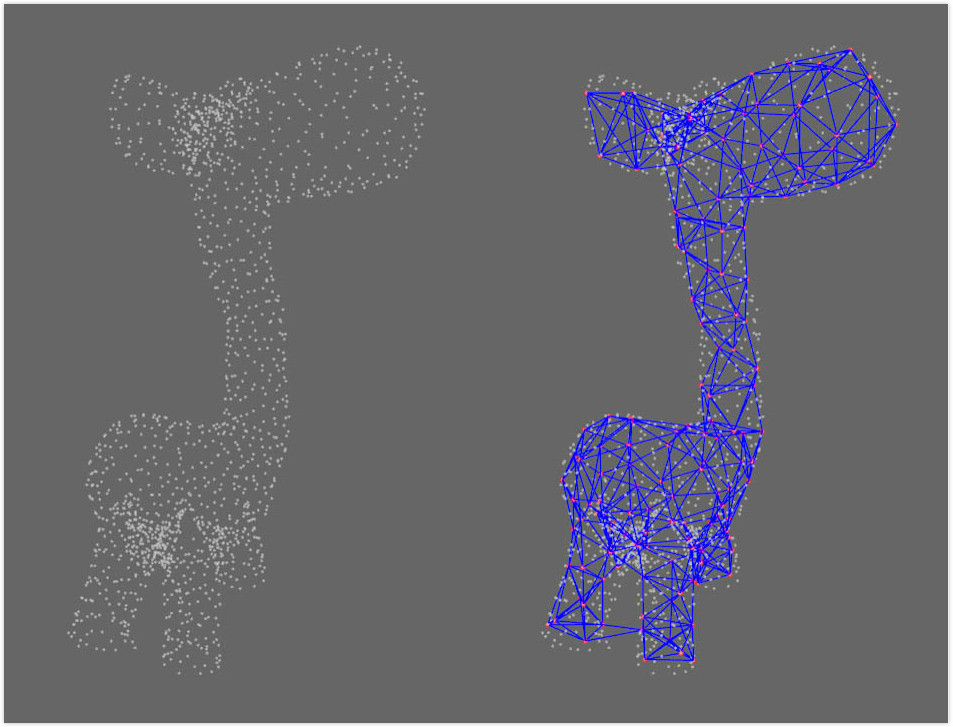
\includegraphics[width = \textwidth]{./Pictures/build_graph.jpg}
    \caption{构建形变图}
    \label{build_graph}
\end{figure}
\begin{algorithm}
    %\fangsong
    \caption{生成形变图边}
    \label{alg_gen_edges}
    \begin{algorithmic}[1]
        \Function {GenerateEdges}{$\bm{Node}$,$k_e$}
            \For{$\forall node_i \in \bm{Node}$}
                % find k-nearest nodes $node_j$ of $node_i$
                %  and build $edge_{ij}$ form $node_i$ to $$
                \For{all $k_e$ nearest nodes $node_j$ of $node_i$}
                    \State $edge_{ij} \gets$ build edge for $node_i$ to $node_j$
                    \State $\bm{Edge} \gets \bm{Edge} \bigcup \{edge_{ij}\}$
                \EndFor
            \EndFor
            \State \Return $\bm{Edge}$
        \EndFunction
    \end{algorithmic}
\end{algorithm} 

构建了形变节点和连接相邻节点的边,形变图本身的结构和性质以及确定,
但还需要确定形变图节点与模型顶点的对应关系,
即确定每个顶点的刚体变换由哪些顶点的刚体变换插值得到。
如同上一节中所说,本文采用k最近邻策略确定控制每个模型顶点的形变节点。
对于模型中的顶点$\bm{v}$,选取形变图中离它最近的$k_v$个形变节点,
作为该节点的控制节点。
在形变过程计算顶点$\bm{v}$发生的刚体变换由它所有的控制节点的刚体形变插值得到。
由于模型顶点和形变图节点的控制关系是通过未发生形变时的位置确定的,
这一关系在形变的过程中并不会改变。
所以控制关系只需要在确定了形变图结构后计算一次并记录下来。
算法\ref{alg_knn_nodes}描述了这一过程。
与生成边的步骤中一样,
k最近邻形变节点可以借助事先构建的KD Tree快速查找。
\begin{algorithm}
    %\fangsong
    \caption{生成形变图边}
    \label{alg_knn_nodes}
    \begin{algorithmic}[1]
        \Function{FindKnnNodesForVertex}{$\bm{Node}$,$\bm{V_{mesh}}$, $k_v$}
            \For{$\forall \bm{v} \in \bm{V_{mesh}}$}
                \State $\bm{Node_{knn}} \gets$ get $k_v$ nearest nodes of $\bm{v}$
                \State $\bm{GN}(\bm{v}) \gets \bm{Node_{knn}}$
            \EndFor
            \State \Return $\bm{GN}$
        \EndFunction
    \end{algorithmic}
\end{algorithm} 

% \begin{algorithm}
%     %\fangsong
%     \caption{形变图构建}
%     \label{alg_build_graph}
%     \begin{algorithmic}[1]
%         \Procedure{BuildGraph}{$\bm{V_{mesh}}$,$r_G$,$k_e$,$k_v$}
%             %\State build KD Tree with $\bm{V_{mesh}}$
%             \State $\bm{Node} \gets$ \Call{GenerateNodes}{$\bm{V_{mesh}}$,$r_G$}
%             %\State build KD Tree with $\bm{Node}$
%             \State $\bm{Edge} \gets$ \Call{GenerateEdges}{$\bm{Node}$,$k_e$}
%             \State $\bm{GN} \gets$ \Call{FindKnnNodesForVertex}{$\bm{Node}$,$\bm{V_{mesh}}$, $k_v$}
%         \EndProcedure
%         \Function{GenerateNodes}{$\bm{V_{mesh}}$,$r_G$}
%             %\State $KDTree \gets$ build KD-Tree with all vertices in $V_{mesh}$
%             \State $\bm{V_{uncovered}} = \bm{V_{mesh}}$
%             \While{$\bm{V_{uncovered}} \neq \varnothing $}
%                 \State $\bm{v_r} \gets$ randomly select a vertex in $V_{uncovered}$
%                 \State $node.\bm{vn} \gets \bm{v_r}$
%                 \State $\bm{Node} \gets \bm{Node} \bigcup \{node\}$
%                 \State $\bm{V_{uncovered}} \gets \bm{V_{uncovered}} - 
%                         \{\bm{v} \in \bm{V_{uncovered}} \quad | \quad 
%                         \|\bm{v} - \bm{v_r}\| \leq r_G\}$
%             \EndWhile
%             \State \Return $\bm{Node}$
%         \EndFunction
%         \Function {GenerateEdges}{$\bm{Node}$,$k_e$}
%             \For{$\forall node_i \in \bm{Node}$}
%                 % find k-nearest nodes $node_j$ of $node_i$
%                 %  and build $edge_{ij}$ form $node_i$ to $$
%                 \For{all $k_e$ nearest nodes $node_j$ of $node_i$}
%                     \State $edge_{ij} \gets$ build edge for $node_i$ to $node_j$
%                     \State $\bm{Edge} \gets \bm{Edge} \bigcup \{edge_{ij}\}$
%                 \EndFor
%             \EndFor
%             \State \Return $\bm{Edge}$
%         \EndFunction
%         \Function{FindKnnNodesForVertex}{$\bm{Node}$,$\bm{V_{mesh}}$, $k_v$}
%             \For{$\forall \bm{v} \in \bm{V_{mesh}}$}
%                 \State $\bm{Node_{knn}} \gets$ get $k_v$ nearest nodes of $\bm{v}$
%                 \State $\bm{GN}(\bm{v}) \gets \bm{Node_{knn}}$
%             \EndFor
%             \State \Return $\bm{GN}$
%         \EndFunction
%     \end{algorithmic}
% \end{algorithm} 
\section{形变参数优化}
在模型表面生成形变图之后,
就可以通过形变图中各节点的参数控制模型的形状。
本文将这些形变节点的参数成为模型的形变参数。
形变捕捉步骤就是通过优化形变参数,
使得模型的形状与深度相机捕捉的物体形状尽可能一致。
\subsection{形变优化流程}
在形变捕捉步骤中,本文的输入是深度视频。
对于视频的每一帧,
本文会优化模型的形变参数。
对于网格模型中的一个顶点$\bm{v_i}$,
它在每一帧的位置位置由两个变换决定。
第一个变换是整个模型在空间中发生的刚体变换$\bm{T_{rigid}}$,
这部分变换被为模型刚体变换;
第二个变换是根据形变图计算出的该节点的变换$G(\bm{v_i}=)Q2T(\hat{\bm{q_{v_i}}})$,
这部分变换被称为模型的非刚体变换。
形变后的模型中顶点的新位置为$\bm{v_i^{'}}=G(\bm{v_i})\bm{T_{rigid}}\bm{v_i}$。
本文需要计算的就是每一帧中的这两个变换。
图\ref{deformation_sampling}描述了形变捕捉的流程。
\begin{figure}
    \centering
    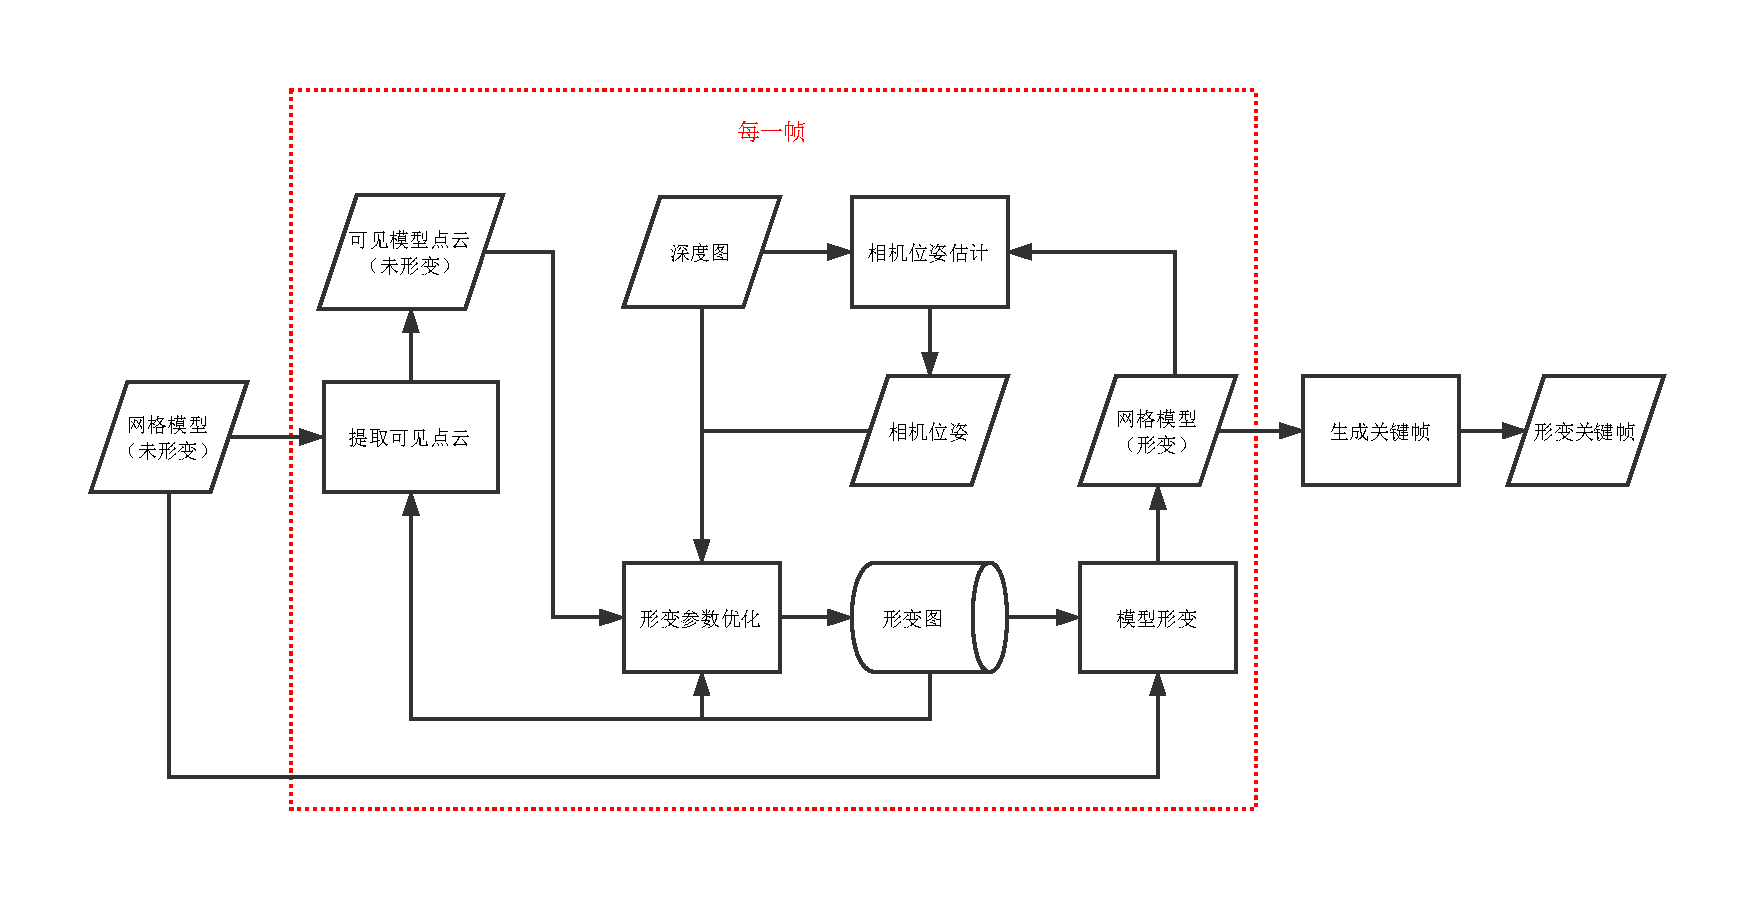
\includegraphics[width = \textwidth]{./Pictures/ds_pipeline_cropped.pdf}
    \caption{形变捕捉流程}
    \label{deformation_sampling}
\end{figure}
首先,本文将根据公式\ref{eq_d2v}将输入的深度图像转换为相应的三维点云。
无论是计算模型的刚体变换还是模型的非刚体变换,
这个点云均被看做模型的参照。

然后,本文会计算当前帧点云相对于上一帧点云的相对刚体变换$\bm{T_{\epsilon }}$。
本文采用ICP算法估计刚体变换$\bm{T_{\epsilon }}$。
ICP算法的输入分别是当前帧的点云,和上一帧形变后的网格模型。 
将ICP计算得到的相对刚体变换叠加到上一帧的上一帧模型刚体变化上,
就能得到当前的模型刚体变换。
\begin{equation}
    \bm{T_{rigid}}=\bm{T_{\epsilon}}\bm{T_{rigid}^{pre}}
\end{equation}
非刚体部分的变换本质上是估计物体和相机的相对位置的变换,
所以图\ref{deformation_sampling}中将这一步骤称为相机位姿估计。

在计算了模型的刚体变换后,本文会优化模型的形变参数,
使得模型在形变后的形状尽量和深度图转换获得的点云接近。
这是一个参数为形变图各节点的双四元数值的最优化问题,
优化的能量函数为:
\begin{equation}
    E(\bm{Node},\bm{Edge},\bm{mesh},\bm{D})=DE(\bm{Node},\bm{mesh},\bm{D})+
    \lambda RE(\bm{Node},\bm{Edge})
\end{equation}
其中,$\bm{D}$为输入的深度图像,$\bm{mesh}$为网格模型;
$\bm{Node}$和$\bm{Edge}$分别为形变图的节点和边的集合;
$DE$为数据能量项,描述了形变后的模型和捕捉到的点云之间的误差;
$RE$为正则项,用来保证形变图的平滑性;
$\lambda$是正则项的权重系数,用来控制形变图中相邻节点间约束的强度;
该优化问题中,优化变量为$\bm{Node}$中各节点中双四元数的值,
关于数据项和正则项的具体形式,下面的章节会做详细的描述。

上述优化的结果将用于更新形变图,
从而改变形变后模型的形状。
如图\ref{deformation_sampling}中所示,
每一帧优化后得到的形变模型将用于估计下一帧的估算相机位姿的输入;
更新后形变图也将用于下一帧分析模型可见性以及数据对应关系的依据。

在形变捕捉的过程中,上述步骤不断重复,
每一帧都会得到一个与深度图像相对应的形变后的网格模型。
本文会从中挑选出一些模型用以构造形变关键帧。
\subsection{数据能量项}
优化形变参数的目标是让形变后的模型形状和深度相机捕捉到的物体形状尽可能接近,
数据能量项就描述了形变后的模型和捕捉到点云之间的误差。

要对两组数据进行比较,首先要确认两组数据间的对应关系。
由于相机只能捕捉到物体朝向相机的那一面的信息,
所以模型中也只有形变后朝向相机的那一部分能有与之对应的深度信息。
这一部分即用深度相机的相机参数对形变后的模型进行三维渲染时被渲染出来的那部分模型,
本文称之为可见模型。
本文会预判模型表面各点在当前帧的可见性,提取出一组可见的点云作为形变图的输入。
对于每一帧,本文都构建了一个从像素坐标到形变模型上对应点在形变前的坐标和法向的映射。
即给定一个像素空间内的坐标$\bm{u}$,能够得到一个顶点坐标$\bm{vo_u}$和法向$\bm{no_u}$,
分别记录了形变模型中投影到像素位置$\bm{u}$处的三维点$\bm{vd_u}$在形变前的位置和法向。
本文会在每一帧计算出一张模型顶点图$\bm{VO}$和一张模型法向图$\bm{NO}$
其尺寸与深度图$\bm{D}$相同,
每个像素分别存储了该像素点对应的初始模型顶点$\bm{VO}(\bm{u})=\bm{vo_u}$
和初始法向$\bm{NO_u}(\bm{u})=\bm{no_u}$,这些点的信息构成了可见模型点云。
这两张图可通过栅格化渲染管线得到。
计算这两张图的过程
可看做渲染形变模型时分别用初始顶点坐标和初始法向作为模型顶点的颜色进行栅格化渲染。
其中的形变模型是根据上一帧更新后的形变图得到的。
此外,如上小结所述,本文还会从当前的深度图生成相应的顶点图$\bm{VD}$,
它的像素中存储了对应的点云顶点位置$\bm{VD}(\bm{u}) = \bm{vd_u}$,
其中$\bm{vd_u}=\bm{D}(\bm{u})\bm{K}^-1[\bm{u},1]$。
数据能量项的定义如下:
\begin{equation}
    DE(\bm{Node},\bm{mesh},\bm{D})=
    \sum \psi_{DE}(
        \hat{\bm{no_u}^T}
        (
            \hat{\bm{vo_u}}
            -
            \bm{vd_{\widetilde{\bm{u}}}}
        )
    )
\end{equation}
其中
\begin{align}
    &\hat{\bm{no_u}}=G(\bm{vo_u})\bm{no_u}=G(\bm{VO}(\bm{u}))\bm{NO}(\bm{u})\\
    &\hat{\bm{vo_u}}=G(\bm{vo_u})\bm{vo_u}=G(\bm{VO}(\bm{u}))\bm{VO}(\bm{u})
\end{align}
分别为可见模型点云根据形变图形变后的顶点坐标与法向量。
$\bm{vd_{\widetilde{\bm{u}}}}$为与其对应的深度图点云$\bm{VD}$中的顶点。
$\widetilde{\bm{u}}$为$\bm{vo_u}$以深度相机的相机参数经过透视投影得到的像素位置。
可以看出$DE$中的每一项是可见点云和深度点云中对应点的连线在模型表面法向上的投影,
即深度点云到中的点到模型表面的距离。
如同DynamicFusion中的数据项,本文采用Tukey惩罚函数提高优化模型的鲁棒性。
$\psi_{de}(f)$即为Tukey惩罚函数:
\begin{equation}
    \psi_{de}(f)= 
    \begin{cases}
        \frac{\epsilon_{de}^2}{6}(1-(1-(\frac{f}{\epsilon_{de}})^3))
        &\quad |f|\leq\epsilon_{de}\\

        \frac{\epsilon_{de}^2}{6}
        &\quad |f|>\epsilon_{de}
        
    \end{cases}
\end{equation}
\subsection{相邻节点约束}
如上一节所说,深度相机只能捕捉到物体朝向相机的那一面的信息。
本文将这一面称为正面,将采集不到的一面称为背面。
模型中只有正面的点才能找到对应的匹配点,
所以也只有位于正面的形变图节点会影响数据能量项的值。

如果优化模型的能量项中只有数据能量项,
优化过程中只有那些影响了数据能量项的节点会被更新,
得到不正确的优化结果。
所以需要在优化模型的能量函数中添加相邻节点间的约束,
使得正面节点的变换能够通过相邻节点间的约束传递到背面。
\begin{equation}
    RE(\bm{Node},\bm{Edge})=
    \sum_{i}^{n}
    \sum_{j \in \bm{Neig}(i)}
    \psi_{re}(
            Q2T(
                \hat{\bm{q_i}}
            )
            \bm{vn_i}
            -
            Q2T(
                \hat{\bm{q_j}}
            )
            \bm{vn_j}
        )
\end{equation}
其中$\bm{Neig}(i)={j \quad | \quad \exists edge_{ij} \in \bm{Edge}}$
包含了所有$node_i$的相邻节点的编号。
可以看出$RE$描述的相邻节点的变换的差别。
添加这一能量项的目的是让优化的结果中相邻节点的变换尽可能接近,
即让局部的变换尽可能的保持刚体变换(As Rigid As Possible),
该约束能够让形变的过程中保持模型的局部特征。
$\psi_{re}(\bm{v})$为Huber惩罚函数,是一个能保持不连续性的惩罚函数
\begin{equation}
    \psi_{re}(\bm{v}) = 
    \begin{cases}
        \frac{1}{2}\|\bm{v}\|^2
        &\quad \|v\| \leq \epsilon_{re}\\
        \epsilon_{re}(\|\bm{v}\|-\frac{\epsilon_{re}}{2})
        &\quad \|v\| > \epsilon_{re}
    \end{cases}
\end{equation}
\section{提取形变关键帧}
\subsection{多视角关键帧合成}
\subsection{关键帧对齐}
\section{本章小结}